\clearpage{\pagestyle{empty}\cleardoublepage}
\lstset{language=erlang, basicstyle=\small\ttfamily, keywordstyle=\color{black}, stringstyle=\color{black}, numbers=left, lineskip=0.4\baselineskip, breaklines=true}
\chapter{Il datacenter}\label{sec:datacenter}
%
Il datacenter \`e il componente del sistema responsabile della elaborazione 
del flusso informativo generato dai dispositivi \emph{di campo} installati 
presso i vari impianti sotto monitoraggio.
%
Si tratta di un sistema software costituito da diverse applicazioni, ciascuna 
delle quali implementa una o pi\`u delle funzionalit\`a tra quelle riportate di seguito:
%
\begin{itemize}
  \item decodifica dei \emph{dati di campo}
  \item stima di grandezze \emph{aggregate}
  \item memorizzazione dei dati su \emph{memoria persistente}
  \item rilevamento di \emph{condizioni anomale} e generazione di \emph{allarmi}
  \item fornire accesso allo \emph{stato} degli impianti
  \item fornire accesso ai \emph{dati storici} degli impianti
\end{itemize}
%

%
Dall'elenco delle funzionalit\`a, \`e facile osservare come il
datacenter ricopra un ruolo fondamentale all'interno del sistema di monitoraggio: 
si tratta di un componente \emph{critico}, un suo malfunzionamento 
(ad esempio uno \emph{shutdown} dovuto a un \emph{crash}) puo` avere effetti che 
vanno dalla semplice interruzione del servizio di accesso ai dati degli impianti 
fino alla mancata decodifica dei dati provenienti dai dispositivi di campo e, 
quindi, al blocco \emph{de facto} dell'intero sistema di monitoraggio.
%
Per questo motivo, durante la prima fase della progettazione, sono stati 
individuati, oltre ai gi\`a elencati requisiti funzionali, un insieme di 
\emph{propriet\`a} di cui il datacenter avrebbe dovuto godere. Tali propriet\`a 
sono:
%
\begin{itemize}
\item \emph{liveness}, i.e. una volta verificatosi un evento di interesse, 
il datacenter deve, prima o poi, gestirlo; tale propriet\`a serve a garantire, ad 
esempio, che ogni \emph{batch} di dati provenienti dai dati di campo venga, 
presto o tardi, processato.
%
\item \emph{high availability}, i.e. il datacenter deve essere costantemente 
in esecuzione, salvo \emph{downtime} programmati per operazioni quali 
aggiornamento release, etc.
%
\item \emph{reliability}, i.e. l'esecuzione del datacenter non deve essere 
compromessa da situazioni anomale quali, ad esempio, la ricezione di dati 
\emph{malformati} da parte di dispositivi di campo in avaria. Il datacenter 
deve essere in grado di rilevare potenziali anomalie.%% e segnalarle?
%
\item \emph{scalability}, i.e. le prestazioni del datacenter non devono 
decrescere all'aumentare del numero di impianti, e, quindi del numero di 
flussi informativi, da monitorare. %% e se un giorno volessi distribuire il datacenter?
%
\end{itemize}
%% dire due parole sul fatto che sono proprieta` note?
%

%
Tali propriet\`a hanno fortemente condizionato il successivo \emph{step} di
progettazione, ovvero la scelta della \emph{tecnologia} su cui costruire il 
datacenter, che \`e, infine, ricaduta su Erlang/OTP.
%

%
Il prossimo paragrafo introdurr\`a OTP, soffermandosi su alcuni dei suoi aspetti 
chiave; il paragrafo successivo analizzer\`a le motivazioni che hanno portato alla 
sua scelta quale piattaforma tecnologica; il resto del capitolo, infine, \`e dedicato 
ad alla descrizione dell'architettura e dei componenti del datacanter.
%

%
\section{Breve introduzione a Erlang/OTP}
%
OTP \`e l'acronimo di \emph{Open Telecom Platform}. Rilasciato da \emph{Ericsson} 
a partire dal 1998, si tratta di un \emph{middleware} per applicazioni distribuite 
scritte in Erlang\cite{erlang}. Il suo campo di applicazione, a dispetto di quanto 
il nome possa lasciar intendere, va ben oltre le telecomunicazioni.
%

%
Una definizione pi\`u articolata di cosa sia OTP \`e fornita da Joe Armstrong in 
\cite{armstrong07}: \emph{OTP is an application operating system and a set of libraries 
and procedures used for building large-scale, fault-tolerant, distributed applications}.
%

%
\subsection{Behaviours}
%
L'intera architettura di OTP si basa sul concetto, fondamentale, di \emph{behaviour}:
un behaviour \`e un componente astratto che implementa un determinato 
\emph{design pattern} tipico della \emph{programmazione concorrente}, p.es. il modello di 
interazione \emph{client/server}. 
%
I behaviour OTP, nel loro complesso, forniscono \emph{a set of standardized building 
blocks used in designing and building industrial-grade systems}\cite{cesarini09}.
%
In altre parole, citando \cite{armstrong07}, il loro utilizzo consente agli sviluppatori 
di concentrarsi sulla parte \emph{funzionale} dell'applicazione, i.e. la \emph{business logic}, 
lasciando che il middleware si occupi di gestire gli aspetti \emph{non funzionali}, quali 
\emph{fault-tolerance}, \emph{scalability}, \emph{dynamic code upgrade}, \emph{inter-process 
communication} ecc.
%

%
I behaviour e i moduli application-specific vanno poi collegati, al fine di definire 
un processo Erlang, mediante l'implementazione di opportune \emph{callback}.
%
\begin{figure}[!h]
\centering
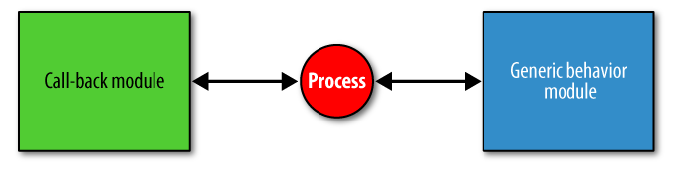
\includegraphics[width=400pt]{img/erl-behaviour.png}
\caption{Processo Erlang costituito da un behaviour e da un modulo di callback}
\end{figure}
%

%
\subsection{Supervision Tree}
%
Esistono due particolari classi di behaviours: \emph{worker} e \emph{supervisor}\cite{otpsupervisor}; 
%
i primi rappresentano i processi che si occupano di effettuare \emph{concretamente} del lavoro, 
p.es. \emph{servers}, \emph{event handlers}, \emph{finite state machines}, ecc.
%
i secondi, invece, si occupano di supervisionare i propri \emph{figli}, i quali possono essere sia
worker che, a loro volta, dei supervisors. 
%
Tra le responsabilit\`a di un supervisor vi sono:
\begin{itemize}
\item \emph{avviare} i processi i figli
\item (opzionalmente) \emph{riavviare} i processi figli in caso di \emph{fault}
\item \emph{terminare} i processi figli al termine dell'applicazione
\end{itemize}
%

%
Il \emph{supervision tree} non \`e altro che una rappresentazione delle relazioni di supervisione 
all'interno di un sistema basato su OTP.
%
\begin{figure}[!h]
\centering
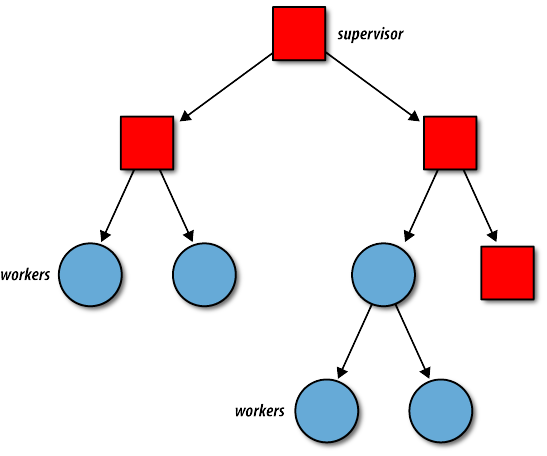
\includegraphics[width=350pt]{img/supervision-tree.png}
\caption{Esempio di supervision tree}
\end{figure}
%

%

%
\subsection{Applications}
%
I supervision tree costituiscono, in un certo senso, lo \emph{scheletro} di ogni applicazione
basata su OTP. Esiste, infatti, un behaviour detto \emph{application}\cite{otpapplication}, 
il cui ruolo \`e quello di raggruppare un insieme di supervision trees, rendendoli 
\emph{riusabili}. 
%

%
In generale, una applicazione OTP \emph{is a reusable component that packages library modules 
together with supervisor and worker processes}\cite{cesarini09}.

%
Una sistema basato su OTP \`e, quindi, formato da un insieme di \emph{application} distribuite 
e \emph{loosely coupled}, ciascuna delle quali implementa una determinata funzionlit\`a.
%

%
\section{Perch\'e OTP}
%
Si \`e scelto di progettare e costruire il datacenter sulla base di Erlang/OTP per i 
seguenti motivi:
%
\begin{itemize}
\item \emph{rapidit\`a di sviluppo}: come gi\`a visto, l'uso dei behaviour consente 
      di concentrarsi sulla business logic di una applicazione; ci\`o \`e particolarmente 
      utile nel caso di applicazioni complesse come il datacenter; 
%% e le caratteristiche 'dichiarative' di Erlang?
%
\item \emph{efficienza e robustezza}: OTP \`e \emph{open source} e, in quanto tale, 
      il suo codice \`e sottoposto a continua revisione e raffinamento; scrivere 
      una applicazione delegando la parte non funzionale a OTP vuol dire, quindi, 
      fare affidamento su una piattaforma assolutamente robusta ed efficiente; 
      a riprova di ci\`o, molti brand famosi utilizzano OTP per alcune delle loro
      soluzioni\cite{whouseserlang}
%
\item \emph{supporto per sistemi sempre online}: i supervisor di un albero possono essere 
      configurati per riavviare i loro worker nel caso in cui questi dovessero, per 
      un qualunque motivo, terminare la loro esecuzione in maniera anormale, i.e. 
      andare in \emph{crash}; ci\`o consente, di fatto, alle applicazioni stesse di
      riavviarsi a seguito di una condizione anomala; OTP elimina persino la necessit\`a
      di mandare offline una applicazione per un \emph{release upgrade}, in quanto 
      supporta l'\emph{hot code swap}
%
\item \emph{rilevamento di crash e recovery}: Erlang pone fortemente l'accento sulla 
      possibilit\`a che i processi possano andare in crash; piuttosto che tentare 
      di prevenire questa eventualit\`a, il linguaggio mette a disposizione gli 
      strumenti necessari per \Item{i} rilevare i crash e \Item{ii} pianificare 
      delle strategie di recupero, e, quindi, per creare sistemi caratterizzati 
      da un elevato grado di \emph{reliability} e \emph{fault tolerance}\cite{armstrongreliability}
%
\item \emph{scalabilit\`a}: uno degli aspetti chiave di Erlang \`e il suo supporto nativo 
      e \emph{sui generis} per la concorrenza; a differenza di altri linguaggi di programmazione, 
      infatti, il modello di concorrenza  implementato da Erlang \`e totalmente indipendente da 
      quello del sottostante sistema operativo, i.e. non esiste un mapping 1-a-1 tra processi 
      Erlang e processi di sistema; ci\`o consente alle applicazioni scritte in Erlang di 
      scalare molto facilmente, come Ghodsi e Armstrong dimostrano in \cite{armstrongyaws}
\end{itemize}
%
%% utilizzo di eunit

%% architettura: insieme di erlang applications:
\section{L'architettura del datacenter}
\label{datacenter-arch}
%
Il datacenter \`e costituito dalle seguenti applicazioni, ciascuna caratterizzata da un 
proprio supervision tree:
%
\begin{itemize}
\item \texttt{database}
\item \texttt{sysconf}
\item \texttt{datamanager}
\end{itemize}
%
Oltre a queste tre applicazioni, il datacenter espone dei web service \emph{RESTful}, 
sfruttando il web server \emph{yaws}\cite{yaws}.
%

%
\section{L'applicazione \emph{database}}
%
Il datacenter si affida a un database MySQL\cite{mysql} per memorizzare in maniera persistente
%
\begin{itemize}
\item la configurazione degli impianti sotto monitoraggio, 
      i.e. quantit\`a, modello e numero di serie dei moduli, numero di stringhe, 
      quantit\`a modello e numero degli inverter, associazioni tra stringa e inverter, ecc.
%
\item le informazioni ricevute dai componenti di campo
\end{itemize}
%
Lo schema relazionale del database \`e mostrato in figura \ref{ermodel}.
%
\begin{figure}[!h]
\centering
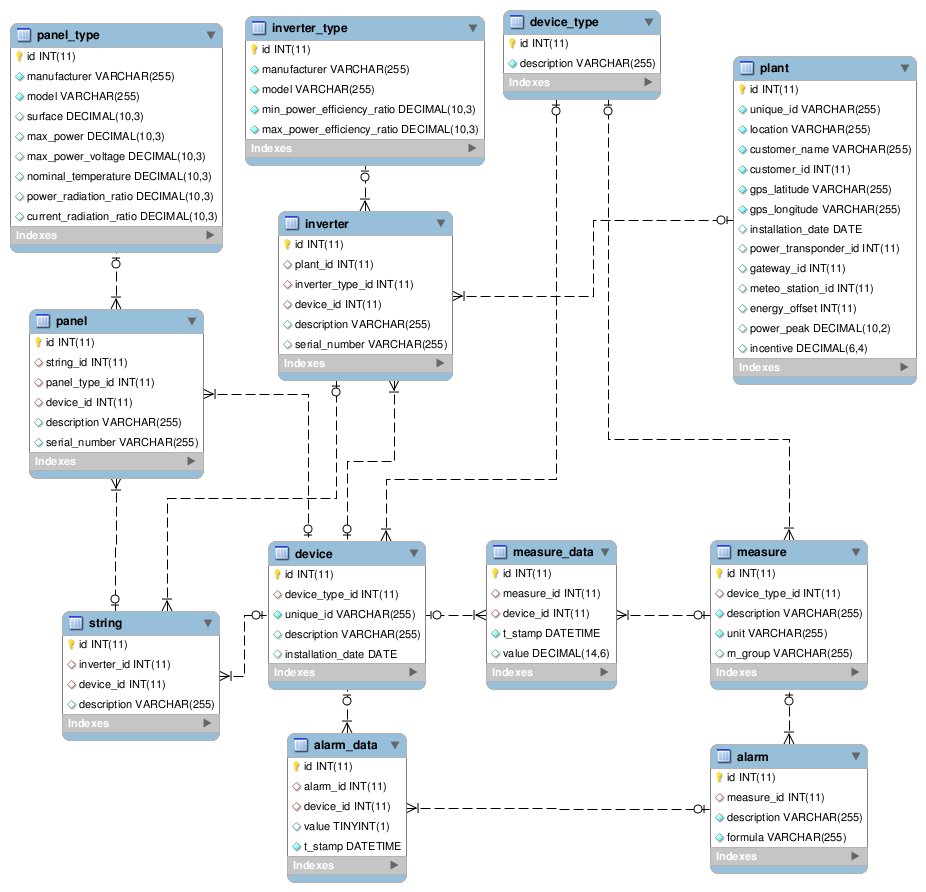
\includegraphics[width=400pt]{img/db-er-model.png}
\caption{Diagramma ER del database}
\label{ermodel}
\end{figure}
%

%
L'applicazione \texttt{database} costituisce, nel contesto del datacenter, 
l'unico punto di accesso alla memoria persistente.
%
Essa \`e interamente basata su \texttt{amnesia}\cite{erl-amnesia}, un wrapper Erlang 
per MySQL, il quale fornisce sia le funzioni per interagire con il database, 
sia gli strumenti necessari a creare dei record erlang per la rappresentazione 
delle entry delle tabelle.
%
In particolare, per le tabelle dello schema relazionale in figura \ref{ermodel}, 
\texttt{amnesia} ha generato i record elencati nel listato \ref{code:database-record}.
%
\begin{lstlisting}[caption={Record per interfacciamento con il database}, label={code:database-record},frame=trBL]
-record (device_type, { ...
-record (device, { ...
-record (measure, { ...
-record (alarm, { ...
-record (inverter_type, { ...
-record (panel_type, { ...
-record (plant, { ...
-record (inverter, { ...
-record (string, { ...
-record (panel, { ...
-record (measure_data, { ...
-record (alarm_data, { ...
\end{lstlisting}
%
Il supervision tree dell'applicazione, mostrato in figura \ref{database-suptree}, \`e molto 
semplice: sono presenti solo \Item{i} un supervisor e \Item{ii} un processo worker, 
\texttt{data\_storage}, il quale implementa il behaviour OTP \emph{gen\_server}\cite{gen-server}.
%

%
\begin{figure}[!h]
\centering
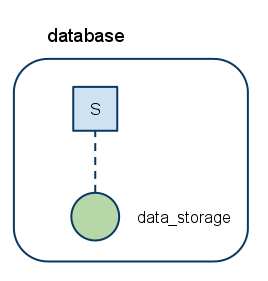
\includegraphics[width=180pt]{img/database.png}
\caption{Supervision tree dell'applicazione Database}
\label{database-suptree}
\end{figure}
%

%
L'interfaccia di \texttt{data\_storage}, le cui funzioni pi\`u importanti sono 
elencate nel listato \ref{code:data_storage_interface}, permettono di:
%
\begin{itemize}
\item aggiungere un impianto
\item modificare la configurazione di un impianto o di uno dei suoi componenti
\item memorizzare i dati di monitoraggio, i.e. il valore delle grandezze monitorate e degli allarmi
\end{itemize}
%

%
\begin{lstlisting}[caption={Interfaccia del modulo \texttt{data\_storage}}, label={code:data_storage_interface},frame=trBL]
-export([%% functions to add new entries
         add_new_device_type/2,
         add_new_inverter_type/3,
         add_new_panel_type/3,
         ...
         add_new_string/2,
         add_new_inverter/2,
         add_new_plant_by_structure/7,
         ...
         set_plant_gateway/4,
         set_string_transponder/6,
         ...    
         %% functions to store monitoring data
         write_variables/1,
         write_alarms/1,
         ...

         %% functions to query the db
         get_plant/1,
         get_plant_structure/1,
         get_plant_devices/1,
         ...
         get_trend_by_device/3
	]).
\end{lstlisting}
%
Il listato \ref{code:new_plant} riporta un esempio di come aggiungere un nuovo impianto
a quelli gi\`a presenti. In particolare, l'esempio mostra come utilizzare la funzione 
\texttt{add\_new\_plant\_by\_structure/7} per aggiungere un impianto costituito da un 
solo inverter a da una sola stringa ad esso connessa.
%
Dopo aver creato il nuovo impianto, mediante la funzione \texttt{set\_plant\_gateway/4}
viene memorizzato sul database anche l'indirizzo fisico del gateway dell'impianto.
%

%
\begin{lstlisting}[caption={Inserimento di un nuovo impianto}, label={code:new_plant},frame=trBL]
%% specify the string configuration
%% i.e., its id and the configuration of each pv module
String = {"String-01", 
          [{"SOVELLO", "SV-X-200", "0000-0000"}]},

%% tell data_storage to create the new plant
data_storage:add_new_plant_by_structure (
      _UniqueID = "MyPlant", 
      _Location = "Nowhere",
      _CustomerName = "Nobody", 
      _Customer_ID = 0,
      _Latitude = "0.0", 
      _Longitude = "0.0",
      %% just one inverter, with the string specified above
      _Inverters = [{{"YURAKU", "I-3000"}, 
                    "Inverter-00", "0000-0000-0000", 
                    [String]} ]),
    
%% set the plant gateway
data_storage:set_plant_gateway (
      _Plant = {unique_id, "MyPlant"}, 
      "E700001A", 
      "", 
      null).
\end{lstlisting}
%

%
\section{L'applicazione \texttt{sysconf}}
%
L'applicazione \texttt{sysconf} fa da supporto all'intero datacenter.
Essa comprende i processi mostrati in figura \ref{sysconfsuptree}.
%
\begin{figure}[!h]
\centering
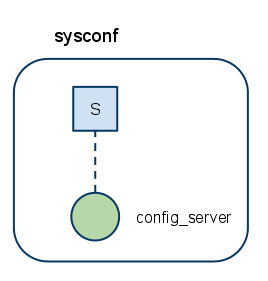
\includegraphics[width=180pt]{img/sysconf.png}
\caption{Supervision tree dell'applicazione Sysconf}
\label{sysconfsuptree}
\end{figure}
%

%
L'unico processo worker presente, \texttt{config\_server}, \`e responsabile della 
gestione e della pubblicazione delle informazioni che costituiscono le configurazioni
dei vari componenti del datacenter. Tali informazioni comprendono,
%
\begin{itemize}
\item le configurazioni dei vari \emph{endpoint} attraverso i quali i gateway possono
      inviare i loro dati al datacenter; p.es. i \emph{path} in cui i \emph{gateway} 
      trasferiscono, via FTP, i file contenenti i dati di campo dei dispositivi;
%
\item le configurazioni dei vari impianti, i.e. quanti e quali dispositivi fanno 
      parte di ogni impianto
\end{itemize}
%
Tali configurazioni sono mantenute nello \emph{stato} del processo: si tratta di un record 
comprendente i seguenti campi:
%
\begin{itemize}
\item \texttt{endpoints\_config}, un record erlang che mantiene le configurazioni dei 
      vari endpoint del sistema
%
\item \texttt{plants}, una tabella che associa, ad ogni impianto, l'elenco dei dispositivi 
      in esso presenti
%
\item \texttt{device\_per\_plant}, una tabella che, dato l'identificatore di un dispositivo,
      permette di risalire all'impianto cui il questo appartiene
\end{itemize}
%

%
La generazione delle configurazioni \`e effettuata durante l'inizializzazione del processo, 
come da listato \ref{code:sysconf-conf-making}.
%
\begin{lstlisting}[caption={Costruzione delle tabelle \texttt{plant} e \texttt{device\_per\_plant}}, label={code:sysconf-conf-making},frame=trBL]
MultiConfigFile = 
  ConfigDir ++ ?MAIN_CONFIGURATION_FILE,

MultiConfigList = 
  conf_manager:load_config(MultiConfigFile),

ParsedConfig = 
  get_configurations(ConfigDir,MultiConfigList),

TableOptions = [set, private, named_table, 
                {read_concurrency, true}],

PlantConfigs = ets:new (plant_configs, TableOptions),
DeviceTable = ets:new (device_table, TableOptions),
    
{ok, Plants} = data_storage:get_plants (),
lists:foreach (
  fun (Plant) ->
      PlantID = Plant#plant.id,
      {ok, Devices} = 
        data_storage:get_plant_devices (PlantID),

      PlantConfig = 
        [I || {#device { unique_id = I}, _, _} <- 
              Devices],

      DeviceEntries = 
        [{I, P} || {#device { unique_id = I}, _, _} <-
                   Devices,
                   P <- [PlantID]],
	      
      ets:insert (PlantConfigs, {PlantID, PlantConfig}),
      ets:insert (DeviceTable, DeviceEntries)
  end, Plants),

State = #config_server_state { config_dir = ConfigDir,
                               config = ParsedConfig,
     		               plants = PlantConfigs,
			       device_per_plant = DeviceTable
			     },
\end{lstlisting}
%

%
Oltre al processo \texttt{config\_server}, il codice della applicazione \texttt{sysconf}
contiene la definizione di un modulo \texttt{logger}, che sfrutta le funzionalit\`a
offerte dalla libreria \emph{log4erl}\cite{log4erl}, al fine di offrire, la possibilit\`a 
di memorizzare su file delle informazioni riguardo il loro stato d'esecuzione.
%

%
\section{L'applicazione \emph{datamanager}}
%
L'applicazione \texttt{datamanager} \`e il componente che si occupa di gestire il flusso 
informativo originato dai gateway degli impianti monitorati, del filtraggio di tali 
flussi informativi, e della memorizzazione dei dati filtrati sul database.
%

%
Rispetto alle altre applicazioni costituenti del datacenter, il \texttt{datamanager} \`e 
caratterizzato da un supervision tree, rappresentato in figura \ref{datamanagersuptree},
pi\`u complesso: esso infatti \`e costituito da un processo \emph{root}, il quale supervisiona
dei \emph{pool}, uno per ogni impianto da monitorare, ciascuno dei quali \`e costituito da un 
supervisor e da due processi worker: un \texttt{filter} e un processo endpoint.
%
Esistono due tipi di endpoint: \texttt{file\_poller} e \texttt{sms\_manager}. Il primo costituisce
l'endpoint di riferimento per i gateway configurati per trasmettere i loro dati mediante 
protocollo FTP, il secondo, invece, per quei gateway che inviano i loro dati mediante \emph{sms}.
%
Si tratta di processi molto simili, motivo per cui, in questa trattazione, daremo spazio solo al
\texttt{file\_poller}.
%

%
\begin{figure}[!h]
\centering
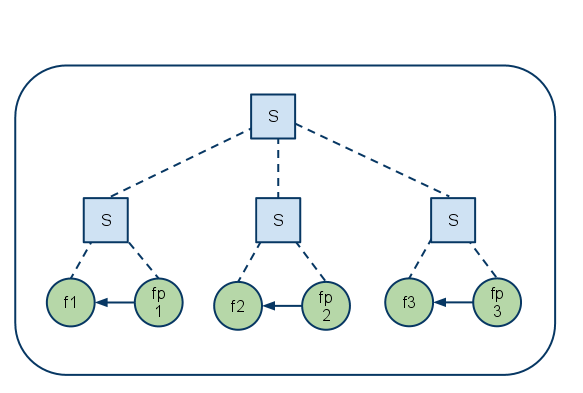
\includegraphics[width=380pt]{img/datamanager.png}
\caption{Supervision tree dell'applicazione Datamanager}
\label{datamanagersuptree}
\end{figure}
%

%
\subsection{Il file\_poller}
%% implementa gen_server
I gateway configurati per l'utilizzo del protocollo FTP inviano al datacenter, 
ad intervalli regolari, un \emph{batch} di file contenenti, ciascuno:
%
\begin{itemize}
\item l'identificatore di un dispositivo di campo
\item un insieme di valori campionati, ciascuno etichettato con un 
      timestamp indicante la data e l'ora del rilevamento
\item informazioni relative allo stato del dispositivo, 
      p.es. lo stato della batteria
\end{itemize}
%
Contestualmente ad ogni \emph{batch}, quale meccanismo di conferma, il gateway invia anche un 
\emph{digest}, riportante l'elenco file inviati.
%

%
Compito del \emph{file\_poller} di un impianto \`e l'effettuazione, ad intervalli di tempo
determinati, delle seguenti operazioni:
%
\begin{enumerate}
\item controlla se il gateway ha trasferito nuovi file; se s\`i,
\item decodifica il digest e leggi l'elenco dei file inviati
\item decodifica il contenuto dei file
\item \emph{passa} le informazioni decodificate al processo \texttt{filter} dell'impianto
\item sposta i file decodificati in un archivio
\item compila dei report riguardo
      \begin{itemize}
      \item eventuali dati non arrivati
      \item eventuali dati \emph{malformati}
      \end{itemize}
\end{enumerate}
%
Questa sequenza di operazioni \`e modellata in figura \ref{fig:polling-sequence} come una
macchina a stati finiti, in cui ogni stato rappresenta una funzione erlang definita nel 
modulo \texttt{file\_poller}.
%
\begin{figure}[!h]
\centering
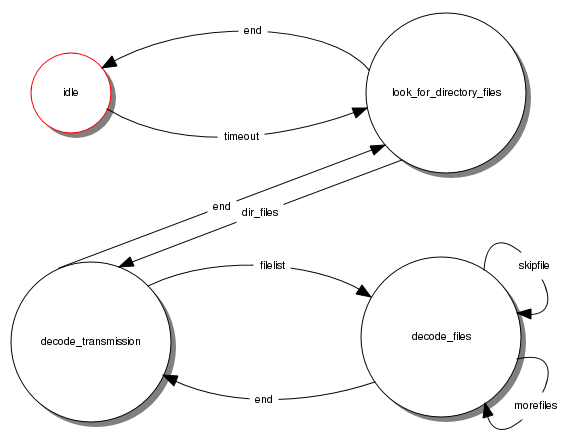
\includegraphics[width=300pt]{img/file-poller.png}
\caption{Sequenza di polling}
\label{fig:polling-sequence}
\end{figure}
%

%
Lo stato \texttt{decode\_files}, all'interno del quale avviene la decodifica dei singoli file,
\`e caratterizzato da due archi \emph{self-connecting}: uno etichettato con \emph{more files}, 
l'altro etichettato con \emph{skip files}.
%
La semantica di queste etichette rispecchia il comportamento della funzione corrispondente 
allo stato \texttt{decode\_files}, riportata nel listato \ref{code:decode_files}. A tale funzione 
va passata la lista dei file da decodificare, lei provveder\`a a decodificarne il primo; quindi, 
se ci saranno ancora \emph{altri file} da decodificare, chiamer\`a se stessa ricorsivamente; 
se la decodifica dovesse fallire (ad esempio perch\`e il formato del file non \`e corretto), 
la funzione \emph{ignorer\`a} quel file e prover\`a a decodificare i rimanenti.
%

%
\begin{lstlisting}[caption={Decodifica dei dati}, label={code:decode_files},frame=trBL]
decode_files ([], Data, State) -> lists:reverse (Data);

decode_files ([File|Rest], Data, State) ->
  Path = State#state.path,
  Result = 
    try
     {ok, FileContent} = 
       file:read_file (lists:concat ([Path, File])),
                       ftp_protocol:decode (FileContent),

     ftp_protocol:decode (FileContent)
		
    catch error : {Reason, D} 
      when (Reason == badmatch) or 
           (Reason == badtimestamp) or
           (Reason == badpreamble) or 
           (Reason == unknown_device_class) -> 
		
      % mark the file as corrupted
      insert_corrupted_file (
        State#state.corrupted_transmissions,
    	{parse_timestamp(File), File}), 
      %% then, return no data
      nil
    end,
    
  case Result of 
    {ok, {DeviceID, DecodedData}} ->
      decode_files (Rest, 
                    [{DeviceID, DecodedData} | Data], 
                    State);
    _->
      decode_files (Rest, Data, State)
  end.
\end{lstlisting}
%

%
Dal listato \ref{code:decode_files} \`e possibile vedere che il \texttt{file\_poller}, rilevato
un file corrotto, invoca la funzione \texttt{insert\_corrupted\_file/2}. Compito di questa funzione 
\`e quello di memorizzare il file corrotto all'interno della \emph{tabella dei file corrotti}, 
i.e. una tabella facente parte dello stato del \texttt{file\_poller}, il cui scopo \`e quello
di tenere traccia dei file corrotti ricevuti.
%

%
Utilizzando lo stesso approccio, il \texttt{file\_poller} tiene anche traccia dei file \emph{missing}, 
i.e. di quei file indicati nei digest inviati dal gateway ma non ricevuti.
%

%
Ad intervalli di tempo determinati, il contenuto delle tabelle viene utilizzato per compilare dei 
\emph{report}, come quello riportato nel listato \ref{code:report-missing-files}, che vengono 
successivamente salvati su file.
%
\begin{lstlisting}[caption={Esempio di report per dati mancanti}, label={code:report-missing-files},frame=trBL]
Received transmission @ {{2011,6,24},{10,18,0}} --> files missing:
    "FFFFFFFF10003000_07DB06180A1200.DAT"
    "FFFFFFFF1000AA00_07DB06180A1200.DAT"
    "FFFFFFFF1000A000_07DB06180A1200.DAT"
    "FFFFFFFF10000300_07DB06180A1200.DAT"
    "FFFFFFFF1000B000_07DB06180A1200.DAT"
    "FFFFFFFF12000500_07DB06180A1200.DAT"
Report generated @ {{2011,6,30},{0,30,40}}
\end{lstlisting}
%

%
Scopo dei report \`e quello di fornire rapidamente delle informazioni precise utili a diagnosticare 
eventuali \emph{fault} di uno qualsiasi dei componenti di campo del sistema di monitoraggio.
%

%
\subsection{La decodifica: \emph{ftp\_protocol}}
%
I file contenenti i dati di monitoraggio inviati dal gateway non hanno tutti lo stesso formato.
%
Esso varia, in generale, a seconda del tipo di dispositivo di campo. Per questo motivo, 
l'operazione di decodifica dei file \`e delegata a un modulo, \texttt{ftp\_protocol}, 
il quale \`e in grado di riconoscere il formato di un file e, quindi, di decodificarlo 
correttamente.
%

%
Le funzioni di decodifica di \texttt{ftp\_protocol} fanno sfruttano la \emph{bit syntax}, una 
sintassi per espressioni Erlang in grado di rappresentare dati binari \emph{raw}.
%
Un esempio d'uso di tali espressioni \`e contenuto nel listato \ref{code:decode-gateway}: si tratta
delle prime righe della funzione \texttt{decode\_gateway\_sample}, il cui compito \`e quello di 
decodificare il singolo campione dati ricevuto da un gateway.
%
\begin{lstlisting}[caption={Decodifica di un blocco dati del Gateway}, label={code:decode-gateway},frame=trBL]
decode_gateway_sample (TemixID, Year, DataBlock, N, Accumulator) ->
    << Battery:2/big-unsigned-integer-unit:8,
       Temperature:2/big-signed-integer-unit:8,
       SolarPanelCurrent:2/big-signed-integer-unit:8,
       Month:8,
       DayOfMonth:8,
       Hour:8,
       Minute:8,
       Rest/binary >> = DataBlock,
       ...
\end{lstlisting}
%

%
\subsection{Il filter}
%% implementa gen_server
Il processo \texttt{filter} si occupa del \emph{filtraggio} dei dati di monitoraggio, i.e.
\begin{itemize}
\item scalare i valori di alcune grandezze, in base alle unit\`a di misura che si desidera
      utilizzare per la loro rappresentazione
%
\item incrementare gli offset delle misure di energia, nel caso venga rilevato un \emph{overflow}
%
\item stimare grandezze \emph{aggregate}
%
\item memorizzare i dati ricevuti sul database
%
\end{itemize}
%
I processi \texttt{filter} lavorano a stretto contatto con gli endpoint di un impianto. 
%
Espongono loro una funzione d'interfaccia, \texttt{put\_variables/4}, mediante la quale 
questi ultimi possono passargli i dati di monitoraggio ricevuti e decodificati.
%

%
Le attivit\`a svolte a \emph{run-time} dal processo \texttt{filter} sono schematizzate in 
figura \ref{filter}: nella parte superiore \`e rappresentata l'attivit\`a di filtraggio 
dei dati di campo; il \emph{triggering event} di questa attivit\`a \`e l'invocazione della 
funzione \texttt{put\_variables/4}.
%
Nella parte inferiore, invece, \`e rappresentata l'attivit\`a di calcolo delle grandezze 
\emph{aggregate}. A differenza della prima, il \emph{triggering event} di questa attivit\`a
\`e sincrono, trattandosi di un evento generato internamente al processo stesso: 
\`e l'azzeramento di un timer locale, configurabile con un parametro \texttt{aggregates\_period}.
%

%
\begin{figure}[!h]
\centering
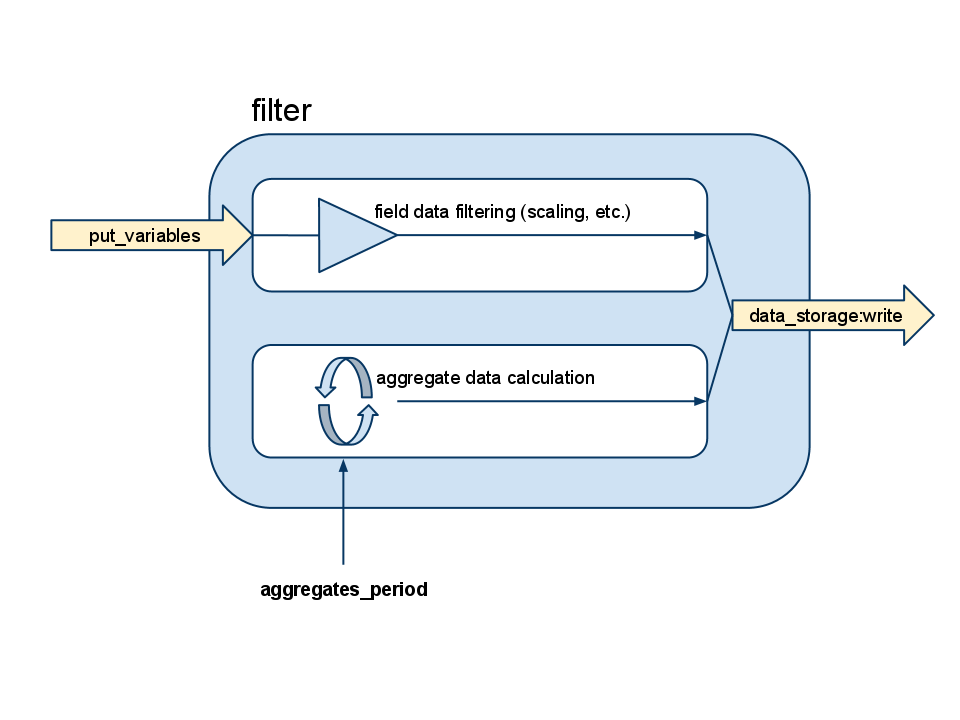
\includegraphics[width=380pt]{img/filter.png}
\caption{Rappresentazione grafica del processo filter}
\label{filter}
\end{figure}
%
Al termine di ciascuna \emph{tranche} di attivit\`a, i dati risultati vengono memorizzati sul 
database, mediante l'invocazione della funzione \texttt{data\_storage:write/4}.
%

%
\subsubsection{Filtraggio dati di campo}
%
Come gi\`a detto, l'attivit\`a di filtraggio dei dati di campo \`e viene effettuata a seguito 
di una invocazione della funzione di interfaccia \texttt{put\_variables}. Tale chiamata viene
\emph{gestita} dal codice riportato nel listato \ref{code:data-filtering}.
%
\begin{lstlisting}[caption={Filtraggio dei dati di campo}, label={code:data-filtering},frame=trBL]
handle_call({put_variables, DateTime, 
             DeviceID, MeasuredVars}, _From, State) ->
    Plant = State#state.plant,

    ScaledVars = scale_vars(DeviceID, MeasuredVars),
    Vars = process_offsets(Plant, DeviceID, ScaledVars),
    data_storage:write_variables([{DateTime, Vars}]),

    {reply, ok, State};
\end{lstlisting}
%

%
Come esempio di filtraggio dati, il listato \ref{code:scale-vars} riporta un frammento della 
definizione della funzione \texttt{scale\_vars/4}. In particolare, si tratta della porzione di 
definizione che si occupa di \emph{scalare} i valori delle grandezze monitorate 
dai Power/Inverter Transponder.
%
Tali conversioni di scala sono necessarie al fine di rendere i dati di campo \emph{consistenti} 
rispetto alle unit\`a di misura con cui il datacenter li rappresenter\`a.
%
\begin{lstlisting}[caption={\emph{Scaling} delle misure del Power Transponder}, label={code:scale-vars},frame=trBL]
scale_vars (_, _, [], Acc) -> lists:reverse(Acc);
%%
scale_vars (DT, ID, [{"current" ++ RN, V} | R], Acc) 
    when (DT == "POWER-TRANSPONDER") or 
         (DT == "INVERTER-TRANSPONDER") ->
    scale_vars (DT, ID, R, 
                [{"current" ++ RN, V / 1000.0} | Acc]);
%%
scale_vars (DT, ID, [{"frequency" ++ RN, V} | R], Acc)
    when (DT == "POWER-TRANSPONDER") or 
         (DT == "INVERTER-TRANSPONDER") ->
    scale_vars (DT, ID, R, 
                [{"frequency" ++ RN, V / 100.0} | Acc]);
%%
scale_vars (DT, ID, [{"voltage" ++ RN, V} | R], Acc)
    when (DT == "POWER-TRANSPONDER") or 
         (DT == "INVERTER-TRANSPONDER") ->
    scale_vars (DT, ID, R, 
                [{"voltage" ++ RN, V / 100.0} | Acc]);
%%
scale_vars(DT, ID, [{"active-power" ++ RN, V} | R], Acc)
    when (DT == "POWER-TRANSPONDER") or 
         (DT == "INVERTER-TRANSPONDER") ->
    scale_vars (DT, ID, R, 
                [{"active-power" ++ RN, V / 100.0} | Acc]);
%%
scale_vars(DT, ID, [{"reactive-power" ++ RN, V} | R], Acc)
    when (DT == "POWER-TRANSPONDER") or 
    (DT == "INVERTER-TRANSPONDER") ->
    scale_vars (DT, ID, R, 
                [{"reactive-power" ++ RN, V / 100.0} | Acc]);
%%
scale_vars(DT, ID, [{"power-factor" ++ RN, V} | R], Acc)
    when (DT == "POWER-TRANSPONDER") or 
         (DT == "INVERTER-TRANSPONDER") ->
    scale_vars (DT, ID, R, 
                [{"power-factor" ++ RN, V / 1000.0} | Acc]);
\end{lstlisting}
%

%
\subsubsection{Calcolo dei valori aggregati}
%
Per ogni dispositivo di campo sono stati definiti dei valori aggregati, i.e. delle 
grandezze stimabili a partire dai dati di campo. 
%
Ad esempio, per i Power/Inverter Transponder sono stati definiti i seguenti due 
aggregati:
%
\begin{itemize}
\item potenza attiva totale, i.e. la somma delle potenze attive rilevate su 
      ciascuna delle tre fasi
\item potenza reattiva totale, i.e. la somma delle potenze reattive rilevate su
      ciascuna delle tre fasi 
\end{itemize}
%

%
Il numero e il nome dei valori aggregati da calcolare per ciascuno dispositivo
sono stati \emph{cablati} nel codice mediante la definizione di funzioni 
come quella riportata nel listato \ref{code:aggregate-definition}.
%
\begin{lstlisting}[caption={Definizione degli aggregati per il Power/Inverter Transponder}, label={code:aggregate-definition},frame=trBL]
power_transponder_aggregates () ->
    ["active-power",
     "reactive-power"].
\end{lstlisting}
%

%
Ovviamente, non basta cablare nel codice il nome degli aggregati, occorre anche 
indicare \emph{come} calcolarli.
%
Per ciascun valore aggregato \`e stata quindi definita una funzione.
%
Il listato \ref{code:aggregate-total-active-power}, ad esempio, riporta il codice 
utilizzato per il calcolo della potenza attiva totale di un power transponder: 
si parte da un istante temporale corrispondente a un campionamento delle variabili di 
campo, \texttt{Timestamp}, e si cercano i valori di potenza attiva rilevati in prossimit\`a
di quell'istante mediante la funzione \texttt{data\_storage:get\_trend\_by\_device}.
%
Una volta ottenuti i valori cercati, la potenza attiva totale \`e calcolata effettuando,
banalmente, lo loro somma.
%
\begin{lstlisting}[caption={Calcolo della potenza attiva totale}, label={code:aggregate-total-active-power},frame=trBL]
{F, T} = get_two_minutes_interval_bounds (Timestamp),
{ok, {_, Vars}} = 
  data_storage:get_trend_by_device (DeviceID, F, T, 
   			           ["active-power-l1",
                                   "active-power-l2",
				   "active-power-l3"]),
	      
PropList = measure_data_to_proplist (Vars),
P1  = proplists:get_value ("active-power-l1", PropList),
P2  = proplists:get_value ("active-power-l2", PropList),
P3  = proplists:get_value ("active-power-l3", PropList),
	      
TotalActivePower = P1 + P2 + P3, 
...
\end{lstlisting}
%

%
\section{Web Services}


%% definizione del wsdl

\begin{lstlisting}[caption={Servizio \texttt{plant\_list}}, label={code:restful-ws},frame=trBL]
<erl>

out(A) ->
  {ok, PlantList} = data_storage:get_plants(),
  Reply = xml_translator:make_plant_list_response (PlantList),
  {html, Reply}.

</erl>
\end{lstlisting}


%% sistemare spazi non devono essere visibili
\begin{lstlisting}[caption={Risposta al servizio \texttt{plant\_list}}, label={code:restful-ws-reply},frame=trBL]
<?xml version="1.0"?>
<plant_list_response>
  <plant id="1" unique_id="plant-1" customer_id="0" customer_name="Customer1" location="Catania" latitude="37.546483" longitude="15.087973"/>
  <plant id="2" unique_id="plant-2" customer_id="1" customer_name="Customer2" location="Roma" latitude="41.782489" longitude="12.448508"/>
</plant_list_response>
\end{lstlisting}


